\section{Programovacie jazyky a kompilátory}
\indent Pri programovacích jazykoch nás zaujímajú ich vyjadrovacie schopnosti ako aj vlastnosti z hľadiska ich rozpoznania. Tieto vlasnosti sa týkajú programovania a prekladu, pričom obe je potrebné zohľadniť pri tvorbe jazyka. V dnešnej dobe sa používajú na programovanie hlavne takzvané vyššie programovacie jazyky, môžeme ich označiť ako zdrojové jazyky. Na to aby vykonávali čo používateľ naprogramoval je potrebné aby boli pretransformované do jazyka daného stroja. Spomínanú transformáciu zabezpečuje prekladač, prekladačom máme na mysli program, ktorý číta zdrojový jazyk a transformuje ho do cieľového jazyka, ktorému rozumie stroj.[1]

\subsection{Proces prekladu}
Aby bol preklad možný, musí byť zdrojový kód programu napísaný podľa určitých pravidiel, ktoré vyplývajú z jazyka. Proces prekladu je možné rodeliť na 4 hlavné časti.
\begin{itemize}
	\item lexikálna analýza
	\item syntakticka analýza
	\item spracovanie sémantiky
	\item generovanie cieľového jazyka
\end{itemize}
\indent Podrobnejšie si stručne popíšeme všetky štyri časti, ktoré majú pre nás z hľadiska prekladu najväčší zmysel.
\newline
\subsubsection{Lexikálna analýza}
	\indent Lexikálna analýza je prvou fázou kompilátora. Dopredu napísaný zdojový kód je postupne spracovávaný preprocesorom, ktorý vytvára takzvané lexémy. 
	 \newline Lexémou nazývame postupnosť alfanumerických znakov. Tieto postupnosti znakov sú následne vkladané do lexikálneho analyzátora, ktorý ma za úlohu vytvoriť zo vstupných lexém tokeny slúžiace ako vstup pre syntaktický analyzátor. 
	 \newline Tokeny sa vytvárajú na základe preddefinovaných pravidiel, ktoré sa v programovacích jazykoch definujú ako pattern. V prípade, že lexikálny analyátor nieje schopný nájsť  pattern pred danú lexému musí vyhlásiť chybu počas tokenizácie.  
	 \newline Výstupom z lexikálnej analýzy sú takzvané tokeny, ktoré tvoria vyššie jednotky jazyka ako kľúčové slová jazyka, konštanty, identifikátory, operátory a iné.
	 
	 \begin{figure}[!htbp]
	 	\centering
	 	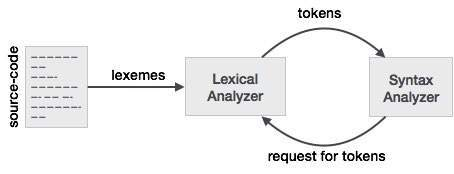
\includegraphics[width=15cm]{img/lexical_analysis.jpg}
	 	\caption{Ukážka práce lexikálneho analyzátora}
	 	\label{fig:test}
	 \end{figure}
 \newline
 
\subsubsection{Syntaktická analýza}
\indent Ďalšou fázou je syntaktická analýza. Úlohou Syntaktického analyzátora je kontrola správnosti vytvorených tokenov s uchovaním niektorých získaných informácií o štruktúre skúmanej syntaktickej jednotky. Syntaktická analýza sa radí medzi bezkontextové gramatiky. Po skoncení syntaktickej analýzy prichádza na rad sémantická analýza.

 \newline
  \newline
\begin{figure}[!htbp]
	\centering
	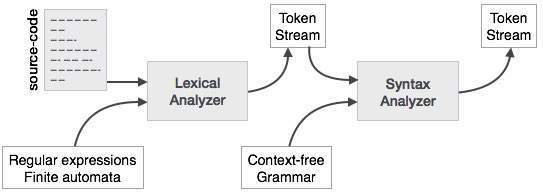
\includegraphics[width=15cm]{img/syntax_analyzer.jpg}
	\caption{Ukážka práce syntaktickeho  analyzátora}
	\label{fig:test}
\end{figure}
 \newline
 \newpage
\subsubsection{Limitácia syntaktickej analýzy}
\indent Syntaktický analyzátor ziska vstup z tokenu, ktorý vytvorí lexikálny analyzátor. Lexikálne analyzátory sú zodpovedné za validitu tokenu.Syntaktické analyzátory majú nasledovné limitácie.

\begin{itemize}
	\item nedokážu zistiť validitu tokenu
	\item nedokážu zistiť či je token používaný pred tým ako je deklarovaný
	\item nedokážu zistiť či je token používaný pred tým ako je inicializovaný
	\item nedokážu zistiť validitu operácie, ktorú token vykonáva
\end{itemize}



\subsubsection{Semantická  analýza}
\indent Sémantická analýza má za úlohu interpretovať symboly, typy, ich vzťahy.Sémantická analýza rohoduje či má syntax programy význam alebo nie.
Ako príklad zisťovania významu môžeme uviesť jednoduchú inicializáciu premennej.

\begin{lstlisting}

	int integerVariable = 6

	int secondIntegerVariable = "six"
\end{lstlisting}

Oba príklady by mali prejsť cez lexikálnu a syntaktickú analýzu. Je až na sémantickej analýze aby rozhodla o správnosti zápisu programu a v prípade nesprávneho zápisu informovala o chybe.  Hlavné úlohy sémantickej analýzy sú" :

\begin{itemize}
	\item zisťovanie dosahu definovaných tokenov takzvaný scoping
	\item kontrola typov
	\item deklaracia premenných
	\item definícia premenných
	\item viacnásobná deklarácia premenných v jedno scope
\end{itemize}

\subsubsection{Generovanie cieľového jazyka}
\indent Generovanie cieľového jazyka môžeme považovať za poslednú fázu kompilátora. V tejto fáze sa preklápa jazyk z vyššieho jazyka do strojového jazyka, ktorý úspešne prešiel cez analyzačné časti .

\subsection{Abeceda a vyhradené slová jazyka}
abeceda jazyka, popis ake pismena-slova rozpoznava, ake su vyhradene slova jazyka a bla bla


\subsection{Procedúry a algoritmy}
procedúra - konečná postupnosť inštrukcií, ktorá sa dá vykonať mechanicky.

\section{Operačné systémy}

\subsection{Windows}
\indent Microsoft Windows uviedol svoje prvé operačné systémy v roku 1985 ako nadstavbu MS DOS. Jeho popularita rýchlo rástla až vyvrcholila dominantným postavením na trhu v osobných počítačoch. V roku 1993 začal vydávať špecializované operačné systémy pre servery, ktoré prinášali novú funkcionalitu pre počítače používané ako servery. Pre účely automatizácie sa na Windows serveroch používajú hlavne powershell scripty, písane v rovnomennom jazyku powershell.
\newline
\subsection{MacOs}
\indent  Mac tiež ponúka serverovú verziu svojho operačného systému pod názvom OS X Server, ktorý začal písať svoju históriu v roku 2001, avšak neteší sa takej obľube ako Windows, unix alebo linux server. Skriptovacím jazykom pre OS X server nieje špecifický jazyk, je možné vybrať si z Pythonu, JavaSriptu, Perl, AppleScriptu, Swiftu alebo napríklad Ruby. Každý jazyk prináša určité plusy, ale zároven mínusy čo je však najpodstatnejšie nie je tam štandardizovaný skriptovací jazyk.
\newline
\subsection{Unix}
\indent Patrí medzi prvé operačné systémy pre servery, ktorých vývoj začal v roku 1970 v priebehu rokov vzniklo nespočetné množstvo nových verzií Unixu. Unixové servery sa tešil veľkej obľube hlavne v minulosti momentálne sú na ústupe hlavne kvoli vyšším nákladom na ich zaobstaranie a prevázku. Pre účely unixu sa vytvoril shell script, oľúbený scriptovací jazyk, ktorý sa v rôznych obmenách teší veľkej obľube medzi administrátormi a automatizačnými programátormi.
\newline
\subsection{Linux}
\indent  Prvé vydanie Linux  bolo 17. septembra 1991, bol rozšírený na najviac platforiem a momentálne sa pýši tým, že je jediný používany operačný systém na TOP 500 superpoťétačoch9(mainframoch) Skriptovací jazyk shell script.
\newline
\section{ Skriptovacie jazyky}
\indent S príchodom počítačov, hlavne serverov, sa programátori zaujímali o automatizáciu procesov, ktoré na danom stoji bolo spočiatku potrebné spúšťať manuálne.
Vačšina serverov bežalo na Unixových distribúciách.

\subsection{Shell}
\indent
Je skriptovacím jazykom pre unixové distribúcie. Počas rokov prešiel roznymi zmenami a rozšíreniami. Verzie shellu su: sh, csh, ksh,tcsh, bash. Bash sa momentálne teši najväčšej obľube no zsh je verzia shellu, ktorá má najviac rôznych rozšírení funkcionality ako aj veľa priaznivcov medzi developermi. V nasledujúcich častiach všeobecne zhodnotíme jednotlivé výhody resp. nevýhody tohoto skriptovacieho jazyka.

\subsubsection{Výhody}
\begin{itemize}
\item automatizácia často opakujúcich sa úloh
\item dokáže zbiehať zloťité zloťené príkazy ako jednoriadkový príkaz  - tzv. reťazenie príkazov
\item ľahký na používanie
\item výborné manuálové stránky
\item ak hovoríme o shell scripte je portabilný naprieč platformami linuxu-unixu
\item jednoduché plánovanie automatických úloh
\newline
\end{itemize}
\subsubsection{Nevýhody}
\begin{itemize}
\item asi najväčšou nevýhodou je ze natívne nefunguje pod windowsom, existuju iba rozne emulátory a 3rd tooly, ktoré sprostredkujú jeho funkcionalitu.
\item pomalé vykonávanie príkazov pri porovnaní s inými programovacími jazykmi
\item nový proces pre skoro každý spustený príkaz
\item zložitejší na pamatanie si rôznych prepínačov, ktoré dané príkazy podporujú
\item nejednotnosť prepínočov(hoc to by asi ani nešlo)
\end{itemize}
\subsubsection{Popis a zhodnotenie jazyka}
\noindent
Shell script je obľúbeným scriptovacím jazykom, vhodným na automatizovanie každodenných operácií. Je jedným z najpoužívanejších skriptovacích jazykou vôbec, nakoľko všetky linuxove, unixové servery využívajú práve tento jazyk ako svoj primárny.
Medzi jeho silné stránky patrí jednoduchá manipulácia s crontable, pomocou ktorej vie admin jednoducho planovať beh procesov.
Avšak syntax jazyka sa učí tažšie nakoľko používa rôzne prepínače, ktoré novému používateľovi nemusia byť sprvu jasné.
V tabuľke uvádzame príklad prepínačov pre if, tiež je vhodné poznamenať, že shell script používa hranaté zátvorky namiesto okrúhlych na aké sme zvyknutý z väčšiny programovacích jazykov. If ponúka aj ďalšie prepínače no zhodnotili sme, že pre ilustráciu budú postačovať aj ukázané.
Najvačsia nevýhoda je, že ani shell script nieje jazyk, ktorý by bol multiplatformový a teda ak by sme mali prostredie, kde servery bežia na rôznych operačných systémoch, potrebujeme poznať ďalší jazyk, ktorým docielime rovnaké alebo aspoň podobné výsledky.
\newline
\begin{table}[h!]
	\centering
	\begin{tabular}{| c | c | }
		\hline
		String Comparison	&Description\\
		\hline
		Str1 = Str2	& Returns true if the strings are equal\\ 
		\hline
		Str1 != Str2 &	Returns true if the strings are not equal\\ 
		\hline
		-n Str1	 &R eturns true if the string is not null\\ 
		\hline
		-z Str1	& Returns true if the string is null\\
		\hline
		\hline
		Numeric Comparison	&Description\\
		\hline
		expr1 -eq expr2	& Returns true if the expressions are equal\\
		\hline
		expr1 -ne expr2	& Returns true if the expressions are not equal\\
		\hline
		expr1 -gt expr2	& Returns true if expr1 is greater than expr2\\
		\hline
		expr1 -ge expr2	& Returns true if expr1 is greater than or equal to expr2\\
		\hline
		expr1 -lt expr2	& Returns true if expr1 is less than expr2\\
		\hline
		expr1 -le expr2	& Returns true if expr1 is less than or equal to expr2\\
		\hline
		! expr1	& Negates the result of the expression\\
	    \hline
	\end{tabular}
\caption{Ukážka prepínačov v podmienkovom výraze if}
\label{table:1}
\end{table}
\newpage

\subsection{Powershel/Classic command line}
\indent
Command line je zakladnym skriptovacim jazykom pre windows distribucie, ktorý poskytuje malé API  pre svojich používateľov. Aj kôli tomu Miscrosoft prišiel s novým jazykom Powershell.

TODO: dpoisat dake sprostosti

Jeho vyhody a nevyhody si popiseme v nasledujujucich castiach.

\subsubsection{Výhody}
\begin{itemize}
	\item bohaté api
	\item výborne riešeny run-time 
	\item flexibilný
	\item veľmi jednoduché prepnúť z .NET
	\newline
\end{itemize}
\subsubsection{Nevýhody}
\begin{itemize}
	\item bohaté api - nejednoznačné, kedy čo použiž
	\item niektoré výhody jazyka sú až nevhodne skryté pred používateľmi
	\item staršie verzie serverov nie sú Powershell-om podporované ako novšie
	\item dokumentácia je horšia ako v prípade Shell scriptu
	\newline
\end{itemize}

\subsubsection{Popis a zhodnotenie jazyka}
bude treba doplniť,

\subsection{JavaScript}
\subsubsection{Výhody}
\begin{itemize}
	\item bohaté api
	\newline
\end{itemize}
\subsubsection{Nevýhody}
\begin{itemize}
	\item nočná mora
	\newline
\end{itemize}

\subsubsection{Popis a zhodnotenie jazyka}
bude treba doplniť,

\subsubsection{Popis a zhodnotenie jazyka}
bude treba doplniť,

\subsection{Gradle}
\subsubsection{Výhody}
\begin{itemize}
	\item bohaté api
	\newline
\end{itemize}
\subsubsection{Nevýhody}
\begin{itemize}
	\item nočná mora
	\newline
\end{itemize}

\subsubsection{Popis a zhodnotenie jazyka}
bude treba doplniť,

\subsubsection{Popis a zhodnotenie jazyka}
bude treba doplniť,

\subsection{Perl}
\subsubsection{Výhody}
\begin{itemize}
	\item bohaté api
	\newline
\end{itemize}
\subsubsection{Nevýhody}
\begin{itemize}
	\item nočná mora
	\newline
\end{itemize}

\subsubsection{Popis a zhodnotenie jazyka}
bude treba doplniť,

\section{Analýza existujucich riešeni}
\indent
Existuje mnozstvo emulatorov a 3rd toolov, ktore sprostredkuvaju funkcionality bashu do windowsu.

Zoznam najlepsich rieseni najdenych na internet:
-cmder- vyuziva ConEmu s vylepseniami clink
-ConEmu
-Babun - poskytuje bash + zsh
-MobaXterm
- ZOC Terminal - ZOC is a professional SSH/telnet client and terminal emulator. With its impressive list of emulations and features, it is a snap to access hosts and mainframes via secure shell, telnet, serial cable, modem/isdn and other methods of communication.
- Console2-  facilitates the running of CMD, PowerShell, Cygwin, PuTTY, etc.g.


\section{Architektúra aplikácie}
\indent Ako sme ukázali existuje veľké množstvo skiptovacích jazykov ci, ktoré dokážu efektívne automatizovať dennodennú prácu avšak majú jeden spoločný nedostatok - nie sú multiplatformové. Táto vlastnosť môže byť  pre niekoho nepodstatná, no pri veľkých projektoch kde sa míňa množstvo prostriedkov na automatizáciu to až tak zanedbateľný fakt nie je. Stačí si len predstaviť koľko času zabere tvorba automatizovaných skriptov pre jednu platformu a pripočítať rovnaké množstvo času pre každú ďalšiu. Niekto by mohol namietať, že pre ďalšie platformy to toľko času nezabere nakoľko logika skriptov je uz definovaná. Tu treba brať ohľad na to, že nie každý jazyk poskytuje programátorovi rovnaké API a teda treba rátať s možnosťou, že niekde bude potrebné doimplementovať veci chýbajúce v jazyku. Preto vyššie spomenuté dôvody sme sa rozhodli pre vytvorenie nového jazyka, ktorý by bol jednoducho rozšíriteľný, manažovateľný, ľahko pisateľný a platformovo nezávislý.

\subsection{Java}
\indent Je vyvíjaný spoločnosťou Oracle. Jeho syntax vychádza z jazykov C a C++. Zdrojové programy sa nekompilujú do strojového kódu, ale do medzistupňa, tzv. „byte-code“, ktorý nie je závislý od konkrétnej platformy. Táto vlastnosť Javy nám veľmi vyhovuje pre dosiahnutie cieľa platformovej nezávislosti. Ďalším veľmi podstatným faktom je, že v Jave programuje veľké množstvo developerov, tým pádom majú open source projekty veľkú šancu, že si ich komunita devoloperov osvojí a prispeje k ich postupnému zlepšovaniu.

\subsubsection{História}
V roku 1991 spoločnosť Sun Microsystems odštartovala tvz. Green project, ktorého cieľom malo byť vytvorenie programovacieho jazyka pre spotrebnú elektroniku. James Gosling ako jeden z hlavných inžinierov tak vytvoril jazyk Oak, ktorý vychádzal zo syntaxe C a C++.

Oak ako programovací jazyk spĺňal podmienku, aby bolo možné program napísať, skompilovať a spustiť na rôznych platformách bez opätovnej rekompilácie, ktorá bola potrebná v prípade jazyka C/C++.

I keď bola Java pôvodne vyvíjaná s cieľom použitia v spotrebnej elektronike, v ktorej Sun videl obrovský potenciál, jej cesta sa celkom nečakane obrátila na web. V dobe rozmachu Internetu boli stránky viac–menej statické a dynamika bola riešená zložitým spôsobom cez CGI skripty vykonávajúce sa na strane servera.

Keďže vývojári webových stránok požadovali možnosť vyššej interaktivity, Gosling so svojím tímom jazyk upravil tak, aby mohol bežať v prostredí webového prehliadača a zabezpečoval potrebnú a požadovanú interaktivitu. Tak vznikli applety, ktoré boli základom ďalšieho úspechu Javy.

Od roku 1995, kedy bola Java oficiálne predstavená, prekonala niekoľko vývojových štádií. Postupne sa prepracovala z klientskej strany na serverovú a jej robustná architektúra si vyslúžila dôveru aj v oblasti bankovníctva a finančníctva. Dnes je možné ju nájsť nielen vo firemnej sfére, ale aj v mobilných telefónoch či komunikačných moduloch.

13. novembra 2006 Sun Microsystems uvoľnil veľkú časť zdrojového kódu Javy pod GNU General Public License (GPLv2). 8. mája 2007 uvoľnil zvyšnú časť kódov, ku ktorým mal na to práva. Reimplementácia zvyšných častí pokračuje.

\subsection{Pouzite navrhove vzory}
Aby sme zaručili rozšíriteľnosť, manažovateľnosť a ďalšie zásady dobrého softwéru bolo potrebné zvoliť vhodnú arhitektúru, ktorú popisujú použité návrhové vzory.
\subsubsection{Command - príkaz}
\indent Command pattern je známy behaviorálny návrhový vzor, používa sa najmä na menežovanie algoritmov, vzťahov a zodpovednosti medzi objektami. 
Cieľom vzoru je zapúzdriť požiadavku(request) ako objekt tým pádom parametrizovať klienta s rôznymi požiadavkami a zabezpečiť operáciu spať.
\begin{figure}[!htbp]
	\centering
	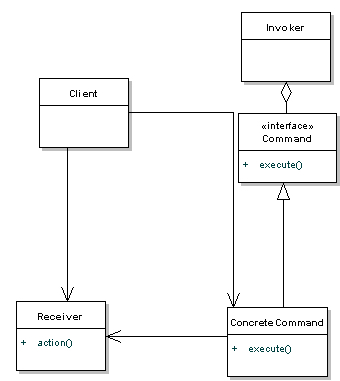
\includegraphics[width=10cm]{img/command_pattern_class.jpg}
	\caption{Class diagram Command návrhového vzoru}
	\label{fig:test}
\end{figure}
\newline
Command vzor deklaruje interface pre všetky budúce commandy a zároveň execute() metódu, ktorú s vypýta Receiver commandu aby splnil požadovanú operáciu.
Receiver je objekt, ktorý vie ako požadovanú operáciu splniť. Invoker pozná command a pomocou implementovanej execute() metódy dokáže vyvolať požadovanú operáciu.
Klient potrebuje implemenotvaž ConcreteCommand a nastavit Receiver pre command. ConcreteCommand definuje spojenie medzi action a receiver. Keď Invoker zavolá execute() metódu na ConcreteCommand spustí tým jednu alebo viac akcií, ktoré budú bežať pomocou Receivera.

Pre lepšie pochopenie je proces zobrazený aj na sekvenčnom diagrame.
\begin{figure}[!htbp]
	\centering
	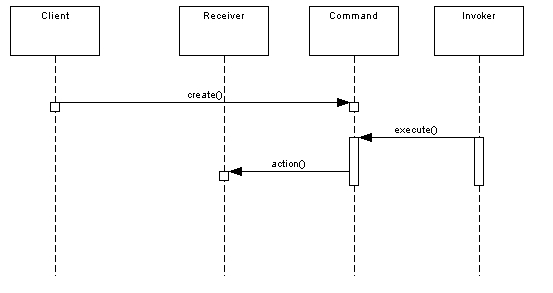
\includegraphics[width=10cm]{img/command_seq.jpg}
	\caption{Sekvenčný diagram Command návrhového vzoru}
	\label{fig:test}
\end{figure}
\newline

\subsubsection{Factory - továreň}
\indent Factory návrhový vzor patrí do sekcie vytváracích vzorov, pomocou tohoto vzoru budeme schopný vytvárať objekty bez toho aby sme prezradili logiku ich vytvárania klientovi.
Diagram návrhového vzoru je mozné vidieť na nasledujúcom obrázku.
\begin{figure}[!htbp]
	\centering
	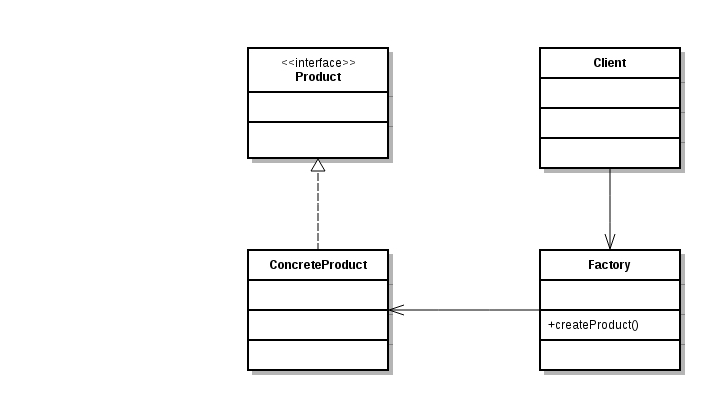
\includegraphics[width=10cm]{img/factory_design_pattern.jpg}
	\caption{Class diagram Factory návrhového vzoru}
	\label{fig:test}
\end{figure}
\newline

\subsubsection{Interpreter}
mozno pouzijem
\subsection{Komponenty aplikácie}
\indent Ako prvé bolo treba zistiť z akých komponentov sa bude aplikácia skladať. Bolo treba zamyslieť sa čo a ako to chceme dosiahnuť. v prvom návrhu sme identifikovali nasledovné komponenty. Rozhodli sme sa, že vytvoríme plugin systém kvôli tomu, čo najdem a napíšem do analyzy.
\begin{itemize}
	\item Parser - vstupov aj vystupov
	\item Loader jar súborov
	\item Sťahovač dependencií - jarka ktoré momentálne produkt neobsahuje napr. cusotm riešenia
	\item Scoping
\end{itemize}

 \begin{figure}[!htbp]
	\centering
	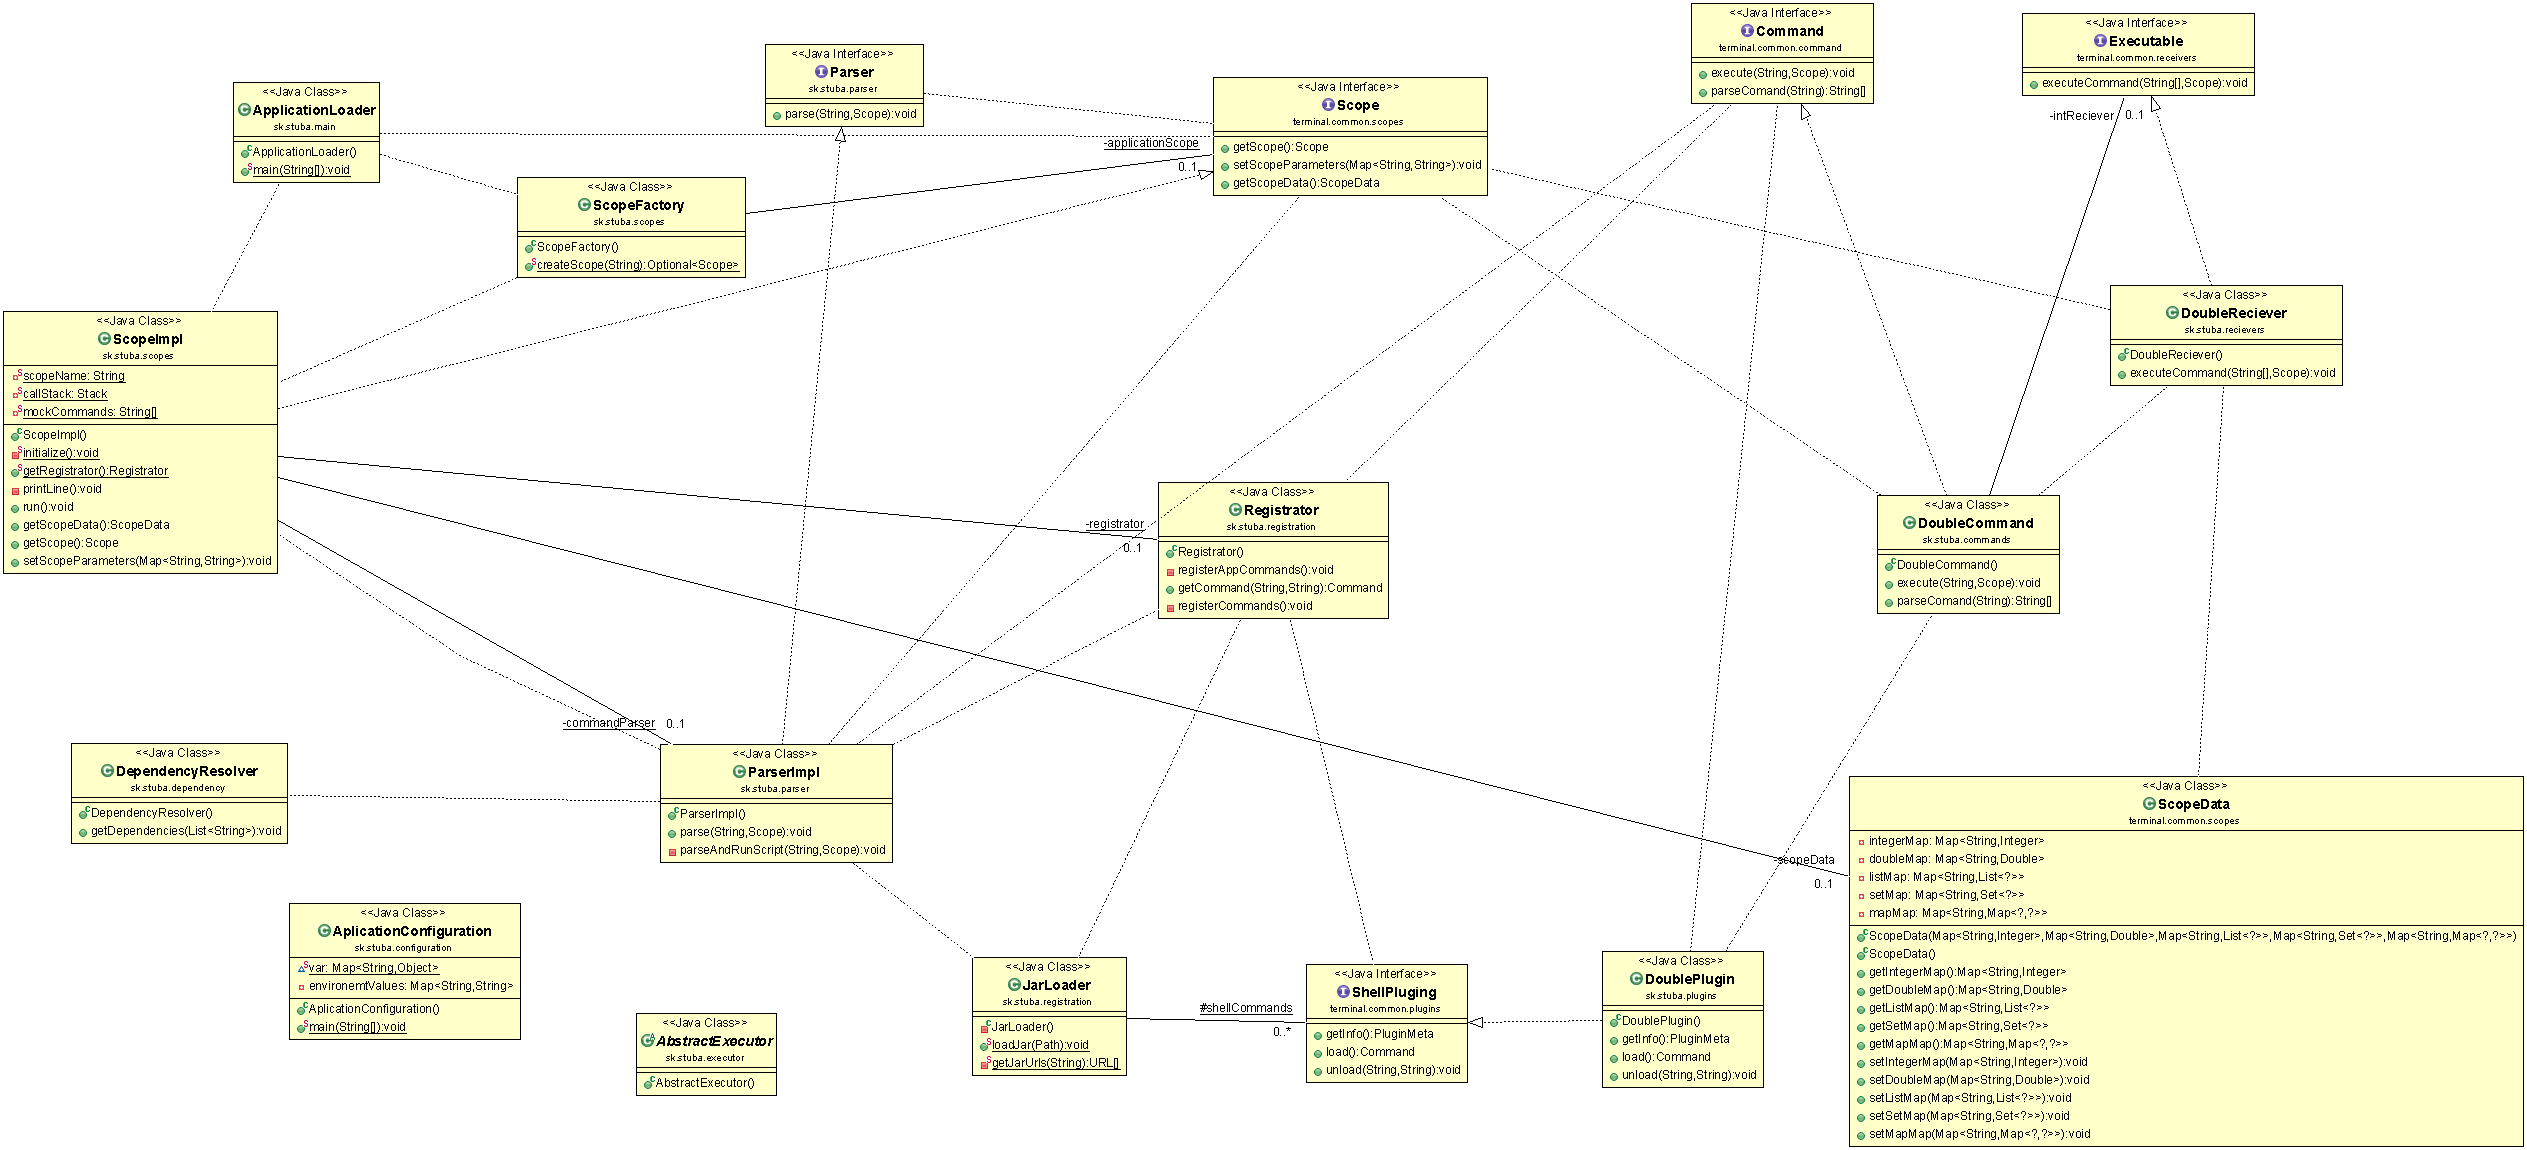
\includegraphics[width=15cm]{img/first_attemp_class_diag.jpg}
	\caption{Pvrvé funkčné riešenie}
	\label{fig:test}
\end{figure}
\newline
Z nasledovného class diagramu nebolo na prvý pohľad zreteľne viditeľné aké komponenty v programe existujú preto bolo potrebné zamyslieť sa ako by sa dali tieto časti rozumne rodeliť. Z prvotného návrhu sme vytiahli plugin. Pre implementáciu pluginu sme sa rozhodli použiť architektúru command patternu. Class diagram implementácie je viditeľný na nasledovnom obrázku.
 \begin{figure}[!htbp]
	\centering
	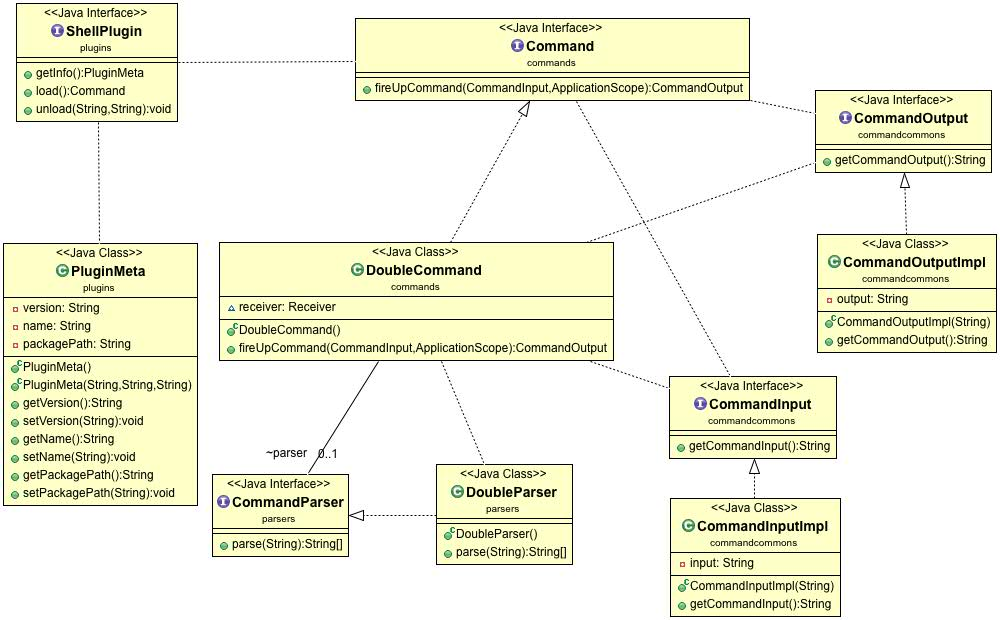
\includegraphics[width=15cm]{img/plugin_class.jpg}
	\caption{Class diagram pluginu}
	\label{fig:test}
\end{figure}
\newline
Popisat scoping
Vytvaranie commandov

\section{Zhodnotenie výsledkov}
Zatiaľ sa toho nespravilo hodne ale verím, že sa to tu cele zaplní.